\documentclass[11pt]{article}

\usepackage[margin=1in]{geometry}
\usepackage{amsmath,amssymb,amsfonts}
\usepackage{graphicx}
\usepackage{hyperref}
\usepackage{natbib}
\usepackage{xcolor}
\usepackage{microtype}
\usepackage{enumitem}
\usepackage{titlesec}
\usepackage{caption}
\usepackage{subcaption}

\graphicspath{{figures/}}

\titlespacing*{\section}{0pt}{1.0em}{0.4em}

\newcommand{\R}{\mathbb{R}}
\newcommand{\norm}[1]{\left\|#1\right\|}
\newcommand{\Ftil}{\widetilde{F}}
\newcommand{\Ytil}{\widetilde{Y}}
\newcommand{\sgn}{\operatorname{sgn}}

\title{\vspace{-2.5em}Spectral Marker of Feature Interaction in\\
Tian's \texttt{Li}$_2$ Grokking Framework\\
{\large \vspace{0.2em} (Technical summary)}}

\author{Yongzhong Xu\\
{\small \texttt{abbyxu@gmail.com}}}
\date{\vspace{-1em}}

\begin{document}
\maketitle
\vspace{-2em}

% ───────────────────────────────────────────────────────────────────────────
\section*{1.\quad Problem}
\vspace{-0.4em}

\citet{tian2025li2} proposes the \texttt{Li}$_2$ framework: grokking in 2-layer
networks $\widehat Y = \sigma(X W) V$ ($\sigma(x) = x^2$, MSE loss with sample-mean
projector $P_1^\perp$) passes through three stages---Lazy, Independent, and
Interactive feature learning---each marked by a different structure of the
backpropagated gradient
\begin{equation}
G_F = -\frac{\partial J}{\partial F} = P_1^\perp (Y - F V) V^\top,
\quad J = \tfrac{1}{2}\norm{P_1^\perp (Y - F V)}_F^2.
\label{eq:gF}
\end{equation}
The framework is mathematically clean. \emph{When} transitions between stages
happen during training is left explicitly uncharacterized.

% ───────────────────────────────────────────────────────────────────────────
\section*{2.\quad Result}
\vspace{-0.4em}

The rolling-window eigengap $\sigma_2/\sigma_3$ of the parameter-update Gram
$\Delta W$ is a clean Stage~III lock-in detector on Tian's exact modular
addition setup ($M=71$, $K=2048$, $n=2016$, Adam at $\text{lr}=10^{-3}$,
weight decay $\eta$). At each epoch we form
\begin{equation}
\Delta := [\Delta W_{t-W+1}, \ldots, \Delta W_t] \in \R^{P \times W},
\qquad
\sigma_k(t) := \lambda_k\!\left(\Delta^\top \Delta\right),
\label{eq:sigma}
\end{equation}
with $W = 20$ (a $W \times W$ eigenproblem; $P = 2M K \approx 2.9\!\times\!10^5$).
A slope detector
\begin{equation}
s(t) := \tfrac{1}{25}\bigl[\log(\sigma_2/\sigma_3)(t) - \log(\sigma_2/\sigma_3)(t-25)\bigr],
\quad \text{``fire''} := \min\{ t \ge 100 : s(t) > 0.04\}
\label{eq:slope}
\end{equation}
gives:

\begin{itemize}[leftmargin=*, itemsep=2pt]
\item Fires at \textbf{median epoch 174 (IQR $=[173,174]$) in 15/15 grok seeds}
($\eta = 2\!\times\!10^{-4}$) and \textbf{0/15 control seeds} ($\eta = 0$).
\item Late-stage magnitude separation: $\sigma_2/\sigma_3 \approx 300$ in grok
vs $\approx 1.31$ in control over epochs 200--400. Cross-condition ratio
$229\times$.
\item Mechanism: between epochs 150 and 200, $\sigma_2$ stabilizes near
$5\!\times\!10^{-3}$ while $\sigma_3$ collapses two orders of magnitude. The
rolling spectrum becomes effectively rank-2.
\end{itemize}

\paragraph{Theorem 6 saturation coincides with the slope-fire moment.}
\citet{tian2025li2} Theorem~6 asserts that for $B := (\Ftil^\top \Ftil + \eta I)^{-1}$
on similar feature pairs,
\begin{equation}
\sgn(B_{j\ell}) = -\sgn\!\left(\widetilde f_j^\top P_{\eta,-j\ell} \widetilde f_\ell\right),
\qquad P_{\eta,-j\ell} := I - \Ftil_{-j\ell}\!\left(\Ftil_{-j\ell}^\top \Ftil_{-j\ell} + \eta I\right)^{-1}\!\Ftil_{-j\ell}^\top.
\label{eq:thm6}
\end{equation}
Approximating $P_{\eta,-j\ell}$ by the full projector $P_\eta$ (relative error
$O(2/K)$ at $K = 2048$) and computing $B$ via Woodbury,
\begin{equation}
B = \tfrac{1}{\eta} I - \tfrac{1}{\eta^2}\Ftil^\top \!\left(\Ftil \Ftil^\top + \eta I\right)^{-1}\!\Ftil
\quad \text{(reduces $K\times K$ inverse to $n\times n$)},
\end{equation}
the empirical sign-match on the top-200 most-similar feature pairs at five
deterministic-replay checkpoints is:

\begin{center}\small
\begin{tabular}{rccccc}
\toprule
epoch & 50 & 100 & \textbf{175} (lock-in) & 250 & 300 \\
\midrule
sign-match & 0.83 & 0.91 & \textbf{0.975} & 0.975 & \textbf{0.995} \\
\bottomrule
\end{tabular}
\end{center}

The sign-rule saturates ($\ge 0.95$) precisely at epoch~175---the same epoch
the $\sigma_2/\sigma_3$ slope detector fires.

% ───────────────────────────────────────────────────────────────────────────
\section*{3.\quad Interpretation}
\vspace{-0.4em}

In Stage III, similar features repel through the negative off-diagonal
entries of $B$. The rolling $\Delta W$ spectrum becomes rank-2 because
two persistent feature directions consolidate while the redundant ones are
pushed out. $\sigma_2/\sigma_3$ is therefore not just \emph{a} late-stage
signature---\textbf{it is a direct observable of Tian's repulsion mechanism
becoming dominant}, with the empirical sign-match providing
the mechanistic verification.

% ───────────────────────────────────────────────────────────────────────────
\section*{4.\quad Negative result}
\vspace{-0.4em}

A simpler signal---the level metric on the activation Gram,
\begin{equation}
\rho_{\mathrm{tian}}(t) := \frac{\norm{P_1^\perp F F^\top - (a I + b\,\mathbf{1}\mathbf{1}^\top)}_F}{\norm{F F^\top}_F},
\label{eq:rho}
\end{equation}
where $a, b$ are empirical diagonal/off-diagonal averages---fires
$\sim 80$ epochs before test accuracy at the $(M=71, \eta=2\!\times\!10^{-4})$
point. An \textbf{$\eta$ sweep} ($\eta \in \{10^{-5}, 5\!\times\!10^{-5},
10^{-4}, 2\!\times\!10^{-4}, 5\!\times\!10^{-4}\}$, five seeds each, 600
epochs) preserves this picture: lead is positive in 20/20 grokking runs
(range 79--154 epochs); $\eta = 10^{-5}$ does not grok and
$\rho_{\mathrm{tian}}$ barely touches the 0.075 threshold.

\begin{figure}[h]
\centering
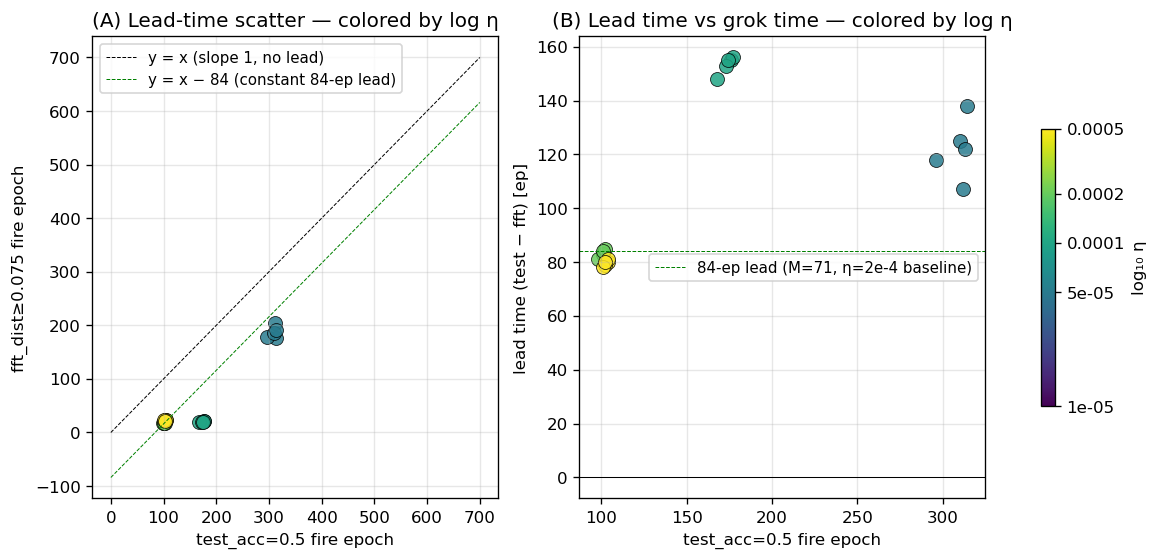
\includegraphics[width=0.95\linewidth]{eta_sweep_scatter.png}
\caption{$\eta$ sweep ($n=25$). Fft fire epoch versus $t_{\text{test}=0.5}$
(left) and lead time versus $t_{\text{test}=0.5}$ (right), colored by
$\log_{10}\eta$. Lead is positive in 20/20 grokking runs.
Linear regression: $t_{\text{fft}} = 0.80\, t_{\text{test}} - 75$
($R^2 = 0.87$).}
\label{fig:eta-sweep}
\end{figure}

\textbf{This survives an $\eta$-sweep but \emph{not} an $M\times p$ scaling
sweep.} On a 60-run sweep ($M \in \{41, 71, 127\}$, $p \in \{0.1, 0.2, 0.3,
0.5\}$, five seeds, $\eta = 2\!\times\!10^{-4}$),
$\rho_{\mathrm{tian}} \ge 0.075$ fires in \textbf{60/60 runs} at near-constant
epoch ($\sim 11$--$25$), including all cells that fail to grok within the
training budget. Across this sweep, fire epoch is decoupled from grokking
outcome.

\paragraph{Reconciliation.} The $\eta$ axis is special: $\eta$ controls
whether feature dynamics happen at all. At $\eta = 0$, the gradient signal
collapses and $\rho_{\mathrm{tian}}$ never crosses threshold. At any
$\eta > 0$ large enough to drive feature dynamics, $\rho_{\mathrm{tian}}$
crosses---at near-constant epoch regardless of whether $(M, p)$ are sufficient
for those dynamics to converge to a generalizable solution. The honest
reading: $\rho_{\mathrm{tian}}$ is a Stage~I$\to$II \emph{initiation}
detector---necessary but not sufficient for grokking. Only the lock-in
detector $\sigma_2/\sigma_3$ survives the full stress test.

% ───────────────────────────────────────────────────────────────────────────
\section*{5.\quad Figure}
\vspace{-0.4em}

\begin{center}
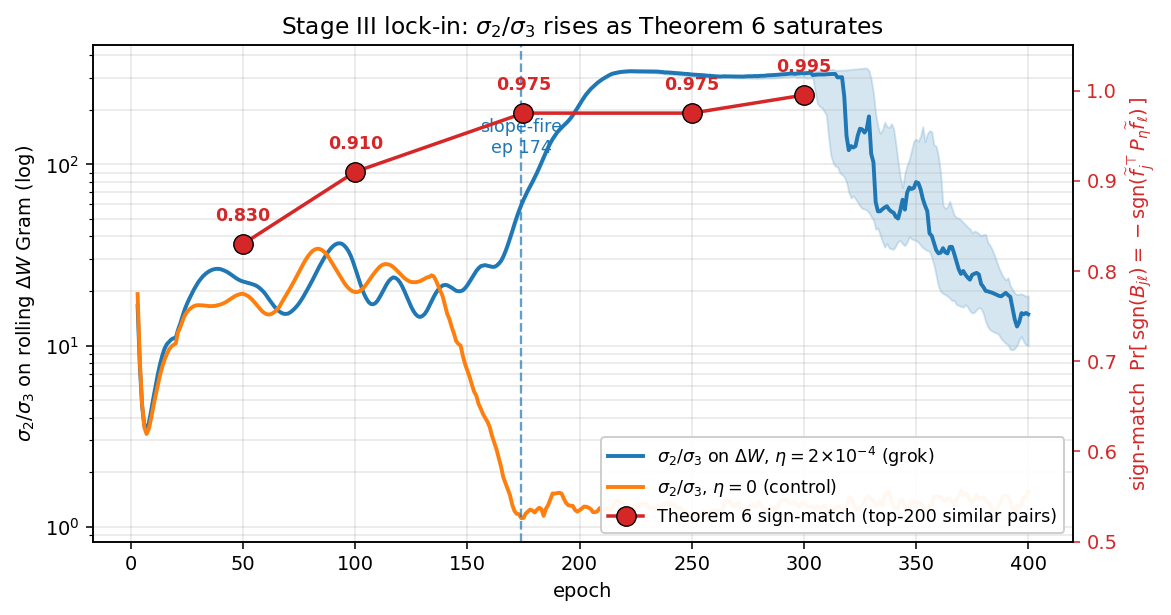
\includegraphics[width=0.95\linewidth]{punch_lockin.png}
\end{center}

\noindent
\textbf{Blue:} median $\sigma_2/\sigma_3$ on rolling $\Delta W$ Gram across
15 grok seeds ($\eta = 2\!\times\!10^{-4}$), with IQR shading and the
slope-fire epoch (174) marked. \textbf{Orange:} median across 15 control
seeds ($\eta = 0$). \textbf{Red:} Theorem~6 sign-match
$\Pr[\sgn(B_{j\ell}) = -\sgn(\widetilde f_j^\top P_\eta \widetilde f_\ell)]$
on top-200 most-similar feature pairs at five deterministic-replay
checkpoints. The $\sigma_2/\sigma_3$ rise to its post-grokking plateau
coincides exactly with Theorem~6 sign-match crossing 0.95.

\bibliographystyle{plainnat}
\bibliography{references}

\end{document}
